\documentclass[onecolumn]{article}
\usepackage[utf8x]{inputenc}
\usepackage{graphicx}
\usepackage{tikz, amsmath, amssymb, bm, color}
\usepackage{geometry}
\usetikzlibrary{calc}
\usetikzlibrary{shapes,arrows}
\usepackage{todonotes}
\usepackage[american]{circuitikz}
\usepackage{pgfplots}
\usepackage{epstopdf}
\usepackage{listings}
\usepackage{subcaption}
\usepackage{mwe}
\usepackage{url}
\usepackage{float}
\usepackage{algorithm}
\usepackage[noend]{algpseudocode}
\usepackage{cleveref}
\usepackage{ragged2e} % For text alignment


\begin{document}


\section*{A hexagon matrix}
\Cref{tkz:hex2matrix} illustates the relationship between the position of an element in a matrix and the location of the hexagon.
\begin{figure}[h]
\centering

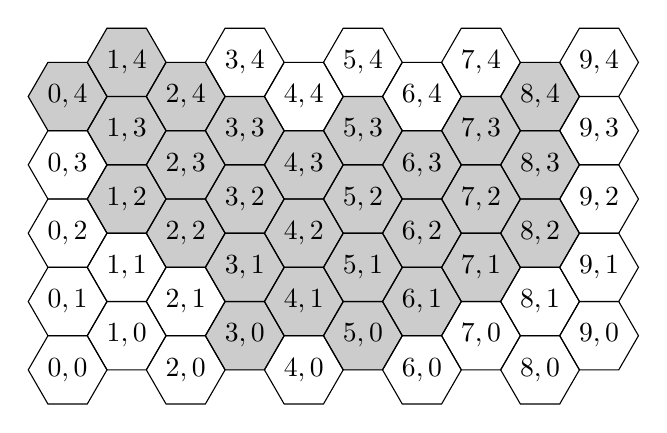
\begin{tikzpicture}[x=7.5mm,y=4.34mm]


 \tikzset{
    box/.style={
      regular polygon,
      regular polygon sides=6,
      minimum size=10mm,
      inner sep=0mm,
      outer sep=0mm,
      rotate=0,
    draw
    }
  }
  

\foreach \i in {0,...,4} 
    \foreach \j in {0,...,4} {
            \node[box] at (2*\i,2*\j) {};
            \node[box] at (2*\i+1,2*\j+1) {};
        }


\node at (0,0) {$0,0$};
\node at (1,1) {$1,0$};
\node at (2,0) {$2,0$};
\node at (3,1) {$3,0$};
\node at (4,0) {$4,0$};
\node at (5,1) {$5,0$};
\node at (6,0) {$6,0$};
\node at (7,1) {$7,0$};
\node at (8,0) {$8,0$};
\node at (9,1) {$9,0$};

\node at (0,2) {$0,1$};
\node at (1,3) {$1,1$};
\node at (2,2) {$2,1$};
\node at (3,3) {$3,1$};
\node at (4,2) {$4,1$};
\node at (5,3) {$5,1$};
\node at (6,2) {$6,1$};
\node at (7,3) {$7,1$};
\node at (8,2) {$8,1$};
\node at (9,3) {$9,1$};

\node at (0,4) {$0,2$};
\node at (1,5) {$1,2$};
\node at (2,4) {$2,2$};
\node at (3,5) {$3,2$};
\node at (4,4) {$4,2$};
\node at (5,5) {$5,2$};
\node at (6,4) {$6,2$};
\node at (7,5) {$7,2$};
\node at (8,4) {$8,2$};
\node at (9,5) {$9,2$};

\node at (0,6) {$0,3$};
\node at (1,7) {$1,3$};
\node at (2,6) {$2,3$};
\node at (3,7) {$3,3$};
\node at (4,6) {$4,3$};
\node at (5,7) {$5,3$};
\node at (6,6) {$6,3$};
\node at (7,7) {$7,3$};
\node at (8,6) {$8,3$};
\node at (9,7) {$9,3$};

\node at (0,8) {$0,4$};
\node at (1,9) {$1,4$};
\node at (2,8) {$2,4$};
\node at (3,9) {$3,4$};
\node at (4,8) {$4,4$};
\node at (5,9) {$5,4$};
\node at (6,8) {$6,4$};
\node at (7,9) {$7,4$};
\node at (8,8) {$8,4$};
\node at (9,9) {$9,4$};

\node [box,fill, opacity=.2] at (4,4) {};
\node [box,fill, opacity=.2] at (3,5) {};
\node [box,fill, opacity=.2] at (2,6) {};
\node [box,fill, opacity=.2] at (3,7) {};
\node [box,fill, opacity=.2] at (4,6) {};
\node [box,fill, opacity=.2] at (5,5) {};
\node [box,fill, opacity=.2] at (5,7) {};
\node [box,fill, opacity=.2] at (6,6) {};
\node [box,fill, opacity=.2] at (7,7) {};
\node [box,fill, opacity=.2] at (8,8) {};
\node [box,fill, opacity=.2] at (7,5) {};
\node [box,fill, opacity=.2] at (8,4) {};
\node [box,fill, opacity=.2] at (7,3) {};
\node [box,fill, opacity=.2] at (6,2) {};
\node [box,fill, opacity=.2] at (5,1) {};
\node [box,fill, opacity=.2] at (4,2) {};
\node [box,fill, opacity=.2] at (3,1) {};
\node [box,fill, opacity=.2] at (5,3) {};
\node [box,fill, opacity=.2] at (6,4) {};
\node [box,fill, opacity=.2] at (3,3) {};
\node [box,fill, opacity=.2] at (2,4) {};
\node [box,fill, opacity=.2] at (1,5) {};
\node [box,fill, opacity=.2] at (2,8) {};
\node [box,fill, opacity=.2] at (1,9) {};
\node [box,fill, opacity=.2] at (0,8) {};
\node [box,fill, opacity=.2] at (1,7) {};
\node [box,fill, opacity=.2] at (8,6) {};
\end{tikzpicture}

\caption{Link between hexagon coordinates and positions in a matrix}
\label{tkz:hex2matrix}
\end{figure}

\begin{figure}[h]
\centering

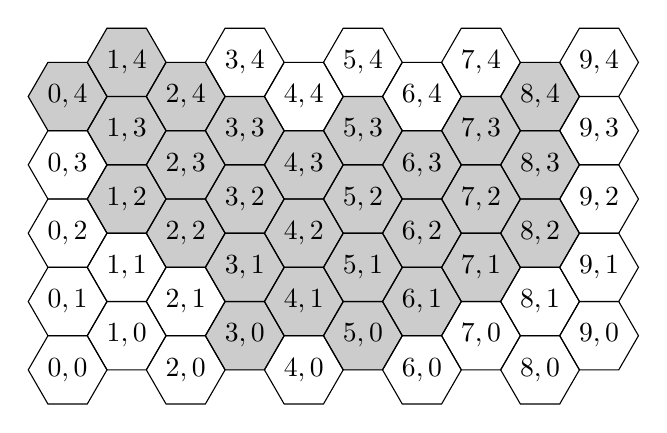
\begin{tikzpicture}[x=7.5mm,y=4.34mm]


 \tikzset{
    box/.style={
      regular polygon,
      regular polygon sides=6,
      minimum size=10mm,
      inner sep=0mm,
      outer sep=0mm,
      rotate=0,
    draw
    }
  }
  

\foreach \i in {0,...,4} 
    \foreach \j in {0,...,4} {
            \node[box] at (2*\i,2*\j) {};
            \node[box] at (2*\i+1,2*\j+1) {};
        }


\node at (0,0) {$0,0$};
\node at (1,1) {$1,0$};
\node at (2,0) {$2,0$};
\node at (3,1) {$3,0$};
\node at (4,0) {$4,0$};
\node at (5,1) {$5,0$};
\node at (6,0) {$6,0$};
\node at (7,1) {$7,0$};
\node at (8,0) {$8,0$};
\node at (9,1) {$9,0$};

\node at (0,2) {$0,1$};
\node at (1,3) {$1,1$};
\node at (2,2) {$2,1$};
\node at (3,3) {$3,1$};
\node at (4,2) {$4,1$};
\node at (5,3) {$5,1$};
\node at (6,2) {$6,1$};
\node at (7,3) {$7,1$};
\node at (8,2) {$8,1$};
\node at (9,3) {$9,1$};

\node at (0,4) {$0,2$};
\node at (1,5) {$1,2$};
\node at (2,4) {$2,2$};
\node at (3,5) {$3,2$};
\node at (4,4) {$4,2$};
\node at (5,5) {$5,2$};
\node at (6,4) {$6,2$};
\node at (7,5) {$7,2$};
\node at (8,4) {$8,2$};
\node at (9,5) {$9,2$};

\node at (0,6) {$0,3$};
\node at (1,7) {$1,3$};
\node at (2,6) {$2,3$};
\node at (3,7) {$3,3$};
\node at (4,6) {$4,3$};
\node at (5,7) {$5,3$};
\node at (6,6) {$6,3$};
\node at (7,7) {$7,3$};
\node at (8,6) {$8,3$};
\node at (9,7) {$9,3$};

\node at (0,8) {$0,4$};
\node at (1,9) {$1,4$};
\node at (2,8) {$2,4$};
\node at (3,9) {$3,4$};
\node at (4,8) {$4,4$};
\node at (5,9) {$5,4$};
\node at (6,8) {$6,4$};
\node at (7,9) {$7,4$};
\node at (8,8) {$8,4$};
\node at (9,9) {$9,4$};

\node [box,fill, opacity=.2] at (4,4) {};
\node [box,fill, opacity=.2] at (3,5) {};
\node [box,fill, opacity=.2] at (2,6) {};
\node [box,fill, opacity=.2] at (3,7) {};
\node [box,fill, opacity=.2] at (4,6) {};
\node [box,fill, opacity=.2] at (5,5) {};
\node [box,fill, opacity=.2] at (5,7) {};
\node [box,fill, opacity=.2] at (6,6) {};
\node [box,fill, opacity=.2] at (7,7) {};
\node [box,fill, opacity=.2] at (8,8) {};
\node [box,fill, opacity=.2] at (7,5) {};
\node [box,fill, opacity=.2] at (8,4) {};
\node [box,fill, opacity=.2] at (7,3) {};
\node [box,fill, opacity=.2] at (6,2) {};
\node [box,fill, opacity=.2] at (5,1) {};
\node [box,fill, opacity=.2] at (4,2) {};
\node [box,fill, opacity=.2] at (3,1) {};
\node [box,fill, opacity=.2] at (5,3) {};
\node [box,fill, opacity=.2] at (6,4) {};
\node [box,fill, opacity=.2] at (3,3) {};
\node [box,fill, opacity=.2] at (2,4) {};
\node [box,fill, opacity=.2] at (1,5) {};
\node [box,fill, opacity=.2] at (2,8) {};
\node [box,fill, opacity=.2] at (1,9) {};
\node [box,fill, opacity=.2] at (0,8) {};
\node [box,fill, opacity=.2] at (1,7) {};
\node [box,fill, opacity=.2] at (8,6) {};
\end{tikzpicture}

\caption{Link from positions in a matrix to hexagon coordinates}
\label{tkz:matrix2hex}
\end{figure}

hoi

$$
ia = 2 \text{mod} 3
$$
\end{document}
